\documentclass[10pt,a4paper,twoside]{article}
\usepackage[english]{babel}
\usepackage{amsmath}
\usepackage{amssymb,amsfonts,textcomp}
\usepackage{subfig}
\usepackage{graphicx}
\usepackage{float,flafter}
\usepackage{cite}
\usepackage{hyperref}
\usepackage[utf8]{inputenc}
\usepackage{float}
\usepackage{pgfplotstable,filecontents}
\setlength\paperwidth{20.999cm}\setlength\paperheight{29.699cm}\setlength\voffset{-1in}\setlength\hoffset{-1in}\setlength\topmargin{1.499cm}\setlength\headheight{12pt}\setlength\headsep{0cm}\setlength\footskip{1.131cm}\setlength\textheight{25cm}\setlength\oddsidemargin{2.499cm}\setlength\textwidth{15.999cm}
\newcommand{\apj}{The Astrophysical Journal}
\begin{document}
	\begin{center}
		\hrule
		\vspace{.4cm}
		{\bf {\huge Subatomic Physics II: Problem set 2}}
		\vspace{.2cm}
		\\
		{\bf Arthur Adriaens}
		\vspace{.2cm}
		\hrule
	\end{center}

\section{The LHC accelerator}
\subsection{fraction of straight sections in the accelerator}
Owing to the Lorentz force $\boldsymbol{v}\times\boldsymbol{B}$, a particle with charge $|q| = e$ has a path described by the formula
\begin{equation}
	p\cos{\lambda} = 0.3\boldsymbol{B}R
\end{equation}
where $\boldsymbol{B}$ is the magnetic flux density in tesla, p is the momentum in GeV/c, R is the radius of curvature in meters and $\lambda$ is the angle between the particle path and the magnetic field. If we take this angle to be zero and rearrange the terms we get:
\begin{equation}
	\frac{p}{0.3B} = R
\end{equation}
Filling in the values for p and $\boldsymbol{B}$ we get R $\approx$ 2791m or a circumference of $\approx$ 17527m which is about 65\% of the real circumference which implies that about 35\% of the accelerator is straights.
\subsection{Amount of collisions in 1 second}
we can take in very good approximation $v\approx c$, if we do this a proton goes about 300000km every second. As the collider is 27km long the proton circles 11111 times every second. As there are 2808 bunches this implies $11111\cdot2808=31.2$MHz ($31.2\times10^{6}$ collision per second).
\subsection{New bunch every 25ns}
Every 25ns implies a frequency of $40$MHz which is not the same for the previous one as the accelerator is not operating at peak crossing rate (an example of a limiting factor is the time it takes for dump kickers to get up).
\subsection{0.58A}
Current is a measurement of charge over time with ampere being measured in coulomb a second. As a proton has an elementary charge which is equal to $e = 1.60217662 \times 10^{-19}$ coulomb, $0.58A = 0.36\times10^{19}$ elementary charges a second or $0.36\times10^{19}\frac{\text{protons}}{s}$. As there pass $31.2\times10^{6}$ bunches a second we get:
\begin{equation}
	\frac{0.36\times10^{19}}{0.312\times10^{8}}\frac{\text{protons}}{\text{second}}\cdot\frac{\text{seconds}}{\text{bunch}} = 1.15\times10^{11}\frac{\text{protons}}{\text{bunch}}
\end{equation}
\subsection{Number of turns proton beam stays in LHC without focussing magnets}
For this we'll take a look at the coulomb repulsion of the protons, the outermost proton of a bunch experiences approximately a force
\begin{equation}
	F = 1.15\times10^{11}\frac{e^2}{4\pi\epsilon_0r^2}
\end{equation}
with r the distance to the other protons (which we assume stay grouped together for simplicity). Now if we take the center of the tube to be x=0 and name the distance to the proton x(t) then we can write:
\begin{equation}
	m_{p}\ddot{x}(t) = 1.15\times10^{11}\frac{e^2}{16\pi\epsilon_0x(t)^2}
\end{equation}
(As the distance to the other part of the bunch is 2x(t)). Now we can write this as
\begin{equation}
	\ddot{x}(t) = \frac{A}{x(t)^2}
\end{equation}
with A $\approx 3.97\times10^9$s$^{-2}$. We now wish to solve for x, for this we can use euler's method and look at what point x becomes 18mm ($1.8\times10^{-2}$):
\begin{figure}[H]
	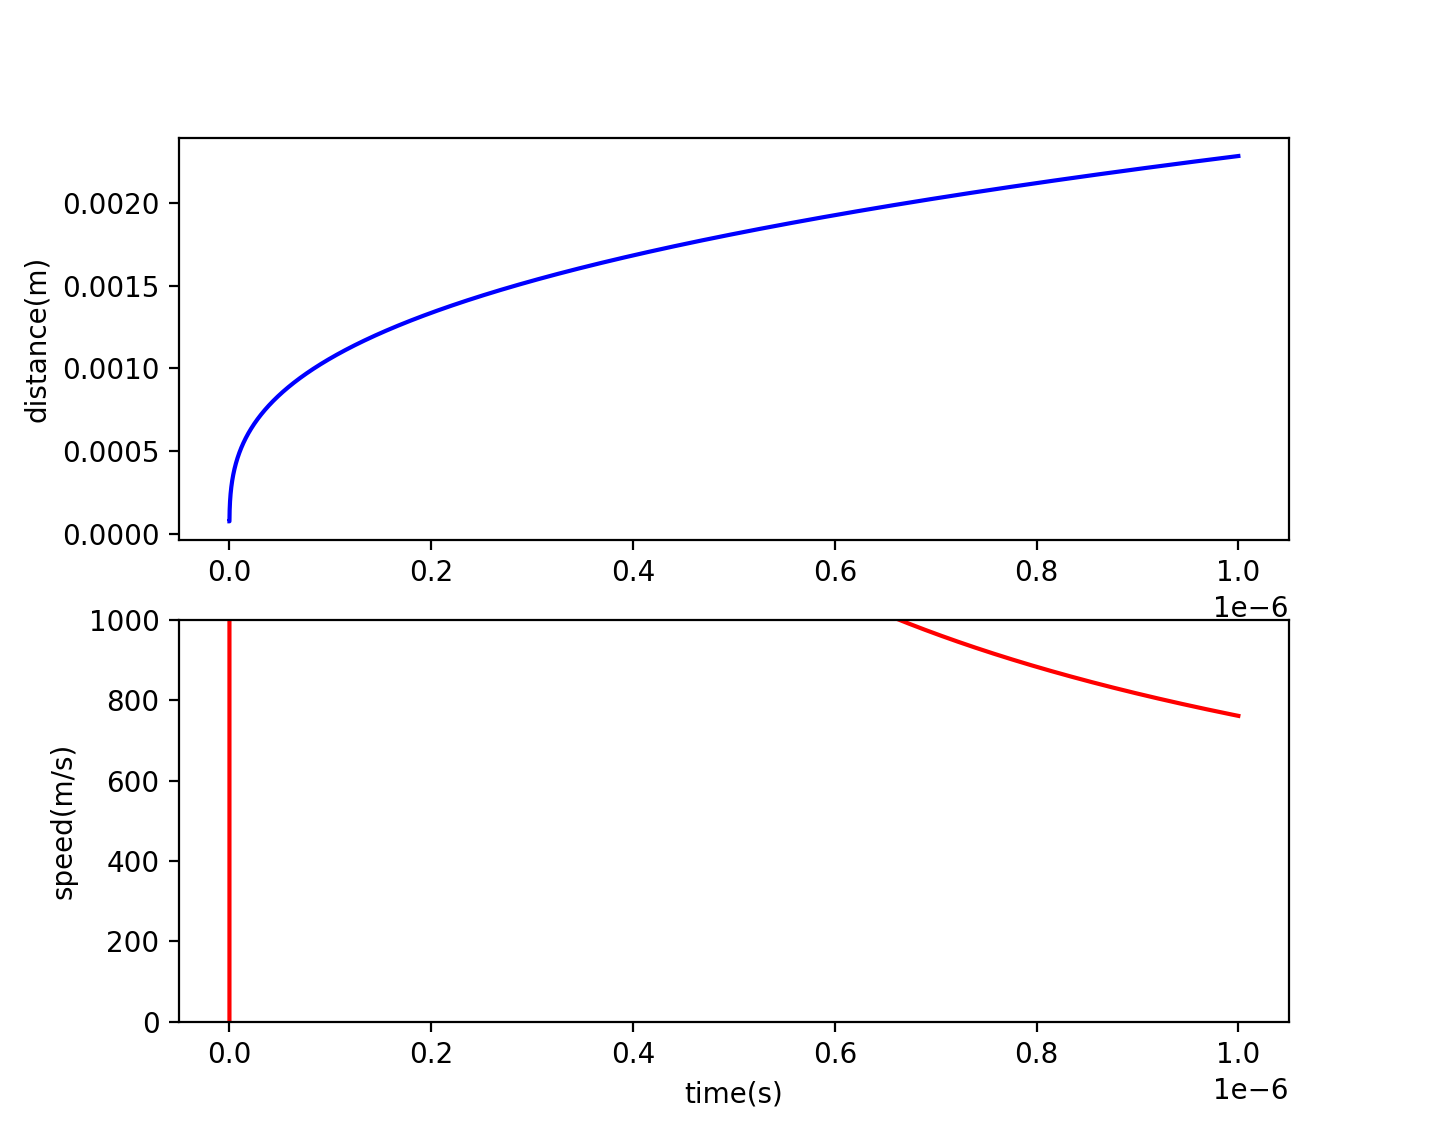
\includegraphics[width=0.5\linewidth]{Figure_1.png}
	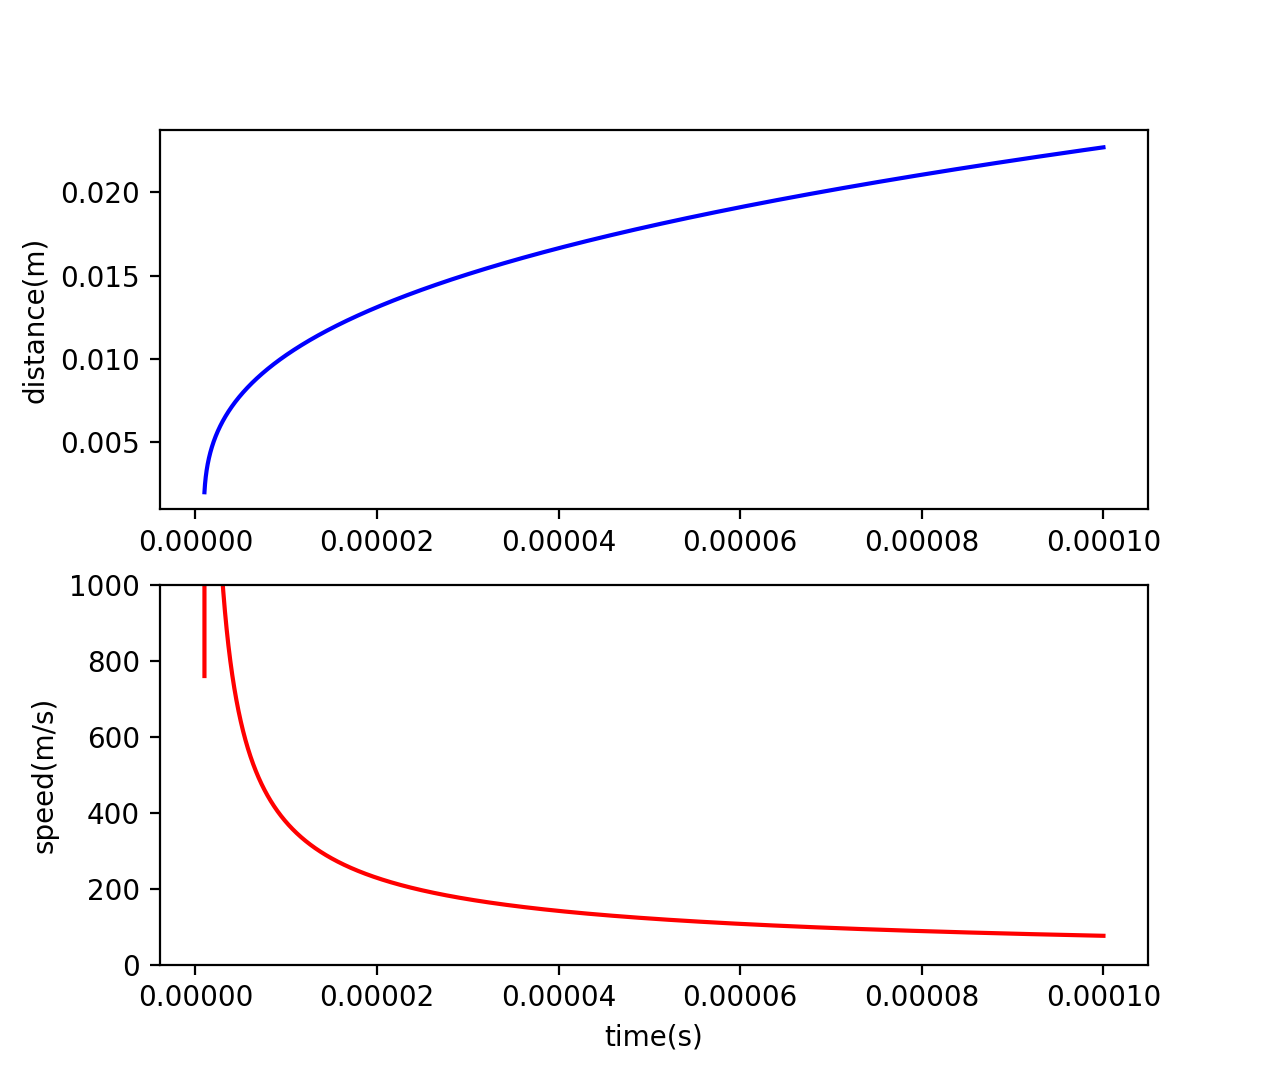
\includegraphics[width=0.5\linewidth]{Figure_2.png}
\end{figure}
\noindent
Where I started at the width of a human hair as that's the quoted bunch width (0.75$\mu$m) resulting in $5\times10^{-5}$s or $300000\cdot5\times10^{-5} = 15$km so not even one rotation.
\section{Mass of the muon-neutrino}
\begin{equation}
	P^{\mu}_{\pi^-} = P^{\mu}_{\mu^-} + P^{\mu}_{\bar{\nu}_{\mu}}
\end{equation}
moving terms we get:
\begin{equation}
P^{\mu}_{\pi^-} - P^{\mu}_{\mu^-} = P^{\mu}_{\bar{\nu}_{\mu}}
\end{equation}
Now multiplying this by itself and the minkowski metric $g_{\mu\nu}$ (using natural units):
\begin{equation}
	m_{\pi^-}^2 + m_{\mu}^2 - 2P^{\mu}_{(\mu^-)}P_{\mu}^{(\pi)} = m_{\bar{\nu}_{\mu}}^2
	\label{neutrino}
\end{equation}
The four-vectors of the particles in the stated system are the following:
\begin{eqnarray}
	P_{\pi^-} &=& (m_{\pi},0,0,0)\\
	P_{\mu} &=& (E_{\mu},p_{\mu},0,0)\\
	P_{\nu} &=& (E_{\nu},-p_{\mu},0,0)
\end{eqnarray}
As there is conservation of three-momentum. Inserting these in equation \ref{neutrino} gives:
\begin{equation}
	m_{\pi^-}^2 + m_{\mu}^2 - 2m_{\pi}E_{\mu} = m_{\nu}^2
\end{equation}
Now, as the muon has a momentum $29.79 \pm 0.01$MeV ($0.034\%$ error), the uncertainty on this value is way bigger than on any mass considered so we can just ignore the other uncertainties. Now as $E = \sqrt{m_{\mu}^2 + p_{\mu}^2}$ we have that: $E_{\mu} \approx 109.78$MeV, now as to know the uncertainty on this value we first seek the uncertainty on $p_{\mu}^2$, this simply follows from
\begin{equation}
	\left(\frac{\sigma_f}{f}\right) = \left(\frac{\sigma_x}{x}\right)^2 + \left(\frac{\sigma_y}{y}\right)^2
\end{equation}
for xy, x/y and y/x. We thus get $\Delta p_{\mu}^2(\%) = \sqrt{2*(3.36\times10^{-4})^2} = 0.048\%$ which gives $\Delta p_{\mu}^2 = 0.42$ as this is $0.0035\%$ of the error under the square root, we finally get that the error on $E_{\mu}$ is $0.0035\% \cdot 109.78 = 0.004$
\begin{eqnarray}
	m_{\nu}^2 &=& (139.57\text{ MeV})^2 + (105.66\text{ MeV})^2 - 2(139.57\text{ MeV})(109.78\pm0.004\text{ MeV})\\
	m_{\nu}^2 &=& 30643.59\text{ MeV}^2 - 30643.42\pm1.07\text{ MeV}^2\\
	m_{\nu} &=& \sqrt{0.16\pm1.07}\text{ MeV}\\
	m_{\nu} &=& 402.71\pm2657\text{ eV}
\end{eqnarray}
\end{document}
